\documentclass[a4paper,11pt]{article}
\usepackage{Settings/style}

\begin{document}
\newcommand{\np}{\newpage}
\newcounter{ProblemCounter}
\renewcommand{\lstlistingname}{Källkod}
% Problem 1
\stepcounter{ProblemCounter}

\pagenumbering{arabic} % Start numbering
\setcounter{figure}{0} % Reset figure numbering
\setcounter{equation}{0} % Reset equation numbering
\setcounter{lstlisting}{0} % Reset code numbering

\begin{center}
    \vspace*{1cm}
    \LARGE
    \textbf{Inlämningsuppgift \arabic{ProblemCounter}}
    
    \Large
    \vspace{0.5cm}
        Fysik - Mekanik och vågor (FAFA01)
    \vspace{0.7cm}
    
    \normalsize
    \textbf{Alexandra Annedotter}
    \\
    \textbf{Georgij Michaliutin}
    
    \vspace{0.5cm}
    Utskriftsdatum: \today
 
    \vspace{1cm}
\end{center}

\section*{\centering Exponentiellt sönderfall}

\subsection*{Teori}

Detta avsnitt grundar sig på kapitel 31.8 och 40 i Tipler och Moscas bok \textit{Physics for Scientists and Engineers} (2008).

Efter att atomer har absorberat energi i form av elektromagnetisk (EM) strålning så emitterar de EM strålning tillbaka. Atomernas emission av EM strälning kallas fluorescens som är kortlivat för de flesta atomer. Antal emitterad fotoner (intensitet $I$) vid angiven tidspunkt $t$ ges av
\begin{equation} \label{eq:I_t}
	I(t) = I_0e^{-t/\tau},
\end{equation}
där $I_0$ är intensiteten då mätningen börjar ($t=0$) och $\tau$ är medellivslängden.

Vid högt antal detekterade fotoner så kan Poissonfördelning approximeras till normalfördelning och ger samma avvikelse $\sigma$ i mätningen av intensiteten.
\begin{equation} \label{eq:I_err}
    \sigma = \sqrt{I}
\end{equation}
Bra empirisk data av emissionsintensiteten ger bra underlag för att hitta tidskonstanten (medellivslängden) för givna atomer. Detta kan göras genom att skriva om ekvation~\ref{eq:I_t} som
\begin{equation} \label{eq:log_I}
	\text{ln}(I(t)) = -\dfrac{t}{\tau} + \text{ln}(I_0)
\end{equation}
och hitta $\tau$ (tidskonstanten) genom linjärisering;
\begin{align}
    k = -\dfrac{1}{\tau} 
    \quad &\Leftrightarrow \quad
	\tau = -\dfrac{1}{k} \label{eq:1_k},
	% b = \text{ln}(I_0) \quad &\Leftrightarrow \quad
	% I_0 = e^{b}
\end{align}
för att sedan beräkna halveringstid $t_{1/2}$ med
\begin{equation} \label{eq:halflife}
    t_{1/2}=\text{ln}(2)\tau.
\end{equation}

\subsection*{Resultat}
Figur~\ref{fig:1_1} presenterar data för observerat antal fotoner.
\begin{figure}[H]
    \centering
    \captionsetup{justification=centering,margin=2cm}
    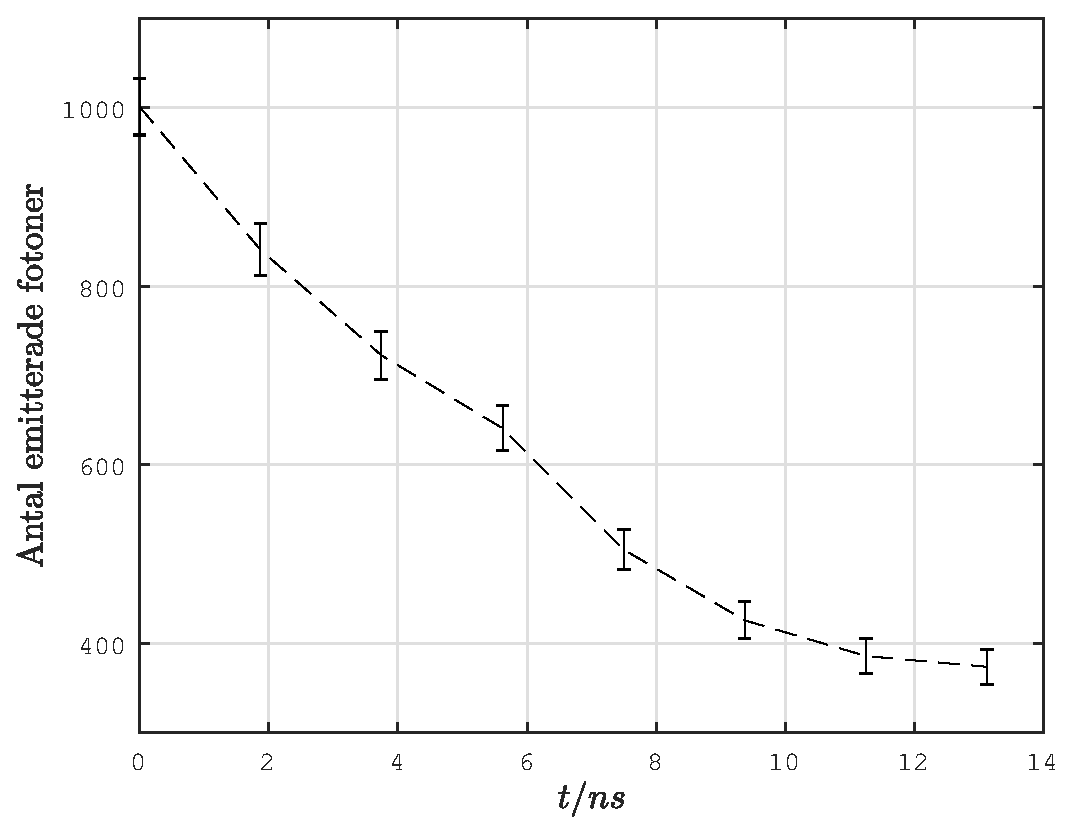
\includegraphics[scale=0.4]{Resources/Graphics/fig1_1.eps}
    \caption{Observerat antal emitterade fotoner inklusive osäkerhet i mätningar.}
    \label{fig:1_1}
\end{figure}

Från Figur~\ref{fig:1_2} beräknades medellivslängd $\tau$ med ekvation~\ref{eq:1_k} till 12.5 ns och halveringstid med ekvation~\ref{eq:halflife} till 8.66 ns. En modell för emissionsintensitet vid en viss tid skapades baserad på resultat och plottades i Figur~\ref{fig:1_3} med observerad data.
\begin{figure}[H]
    \minipage{0.47\textwidth}
        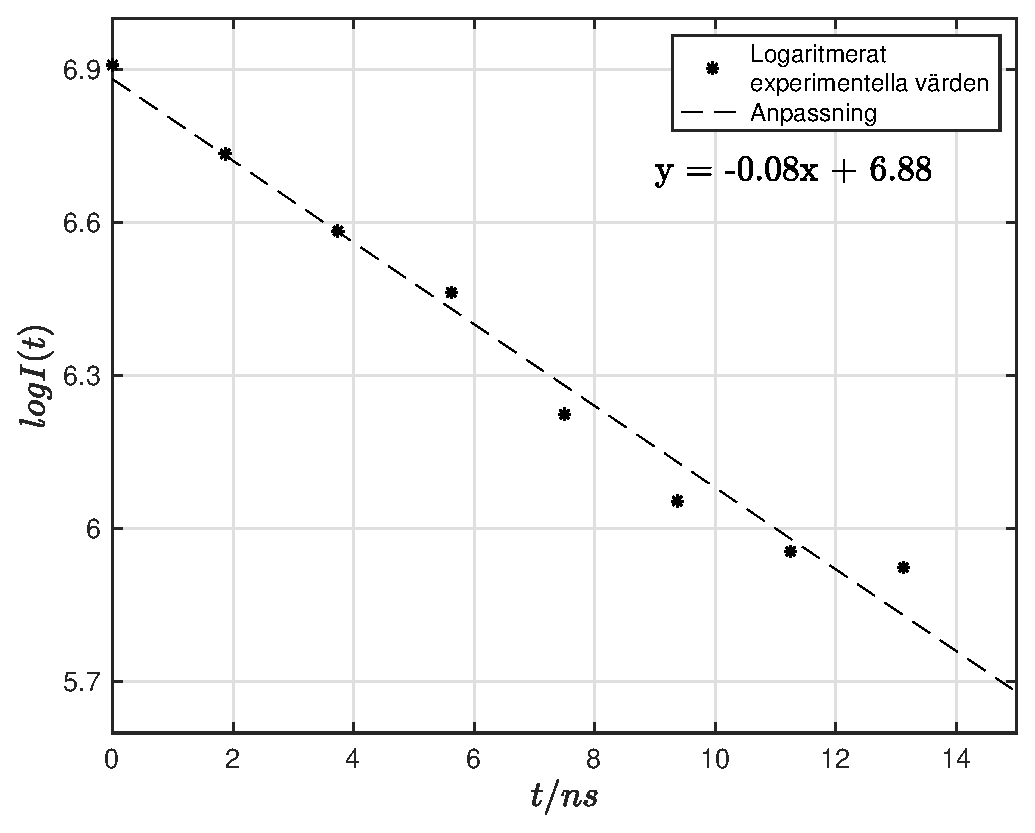
\includegraphics[width=\linewidth]{Resources/Graphics/fig1_2.eps}
        \caption{Linjärisering av data från Figur~\ref{fig:1_1}}\label{fig:1_2}
    \endminipage\hfill
    \minipage{0.47\textwidth}
        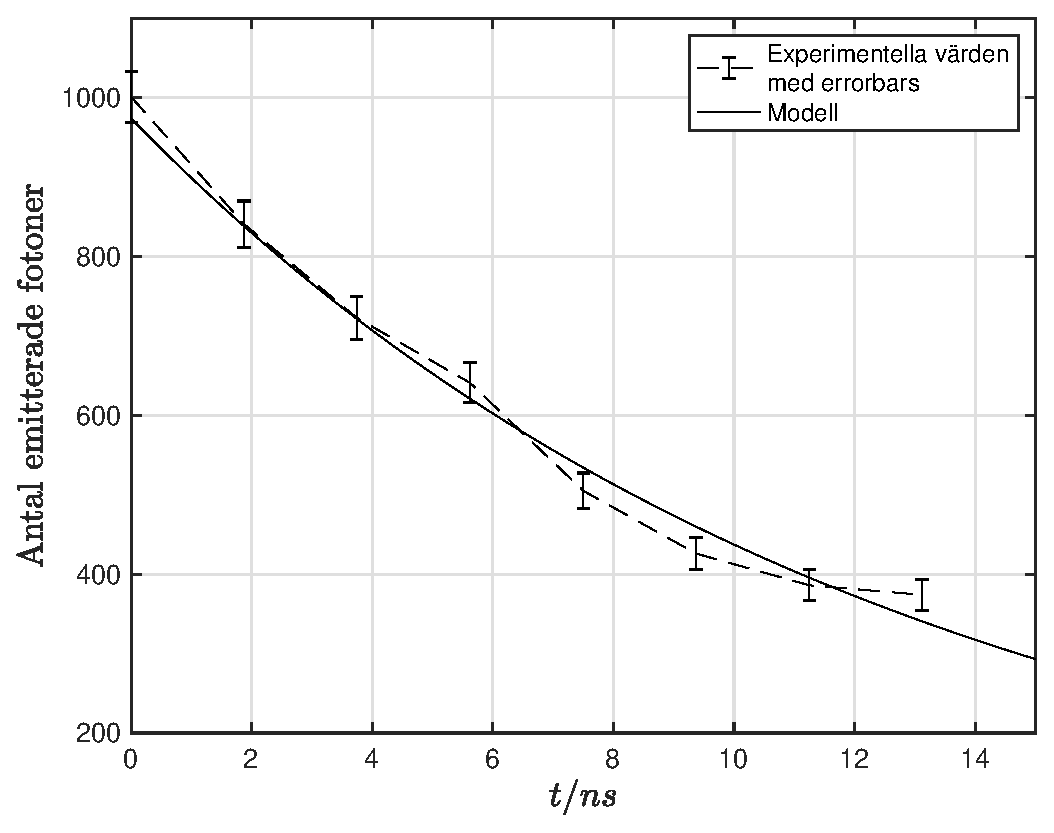
\includegraphics[width=\linewidth]{Resources/Graphics/fig1_3.eps}
        \caption{Observerad data och en modell för tidskonstanten}\label{fig:1_3}
    \endminipage
\end{figure}

\subsection*{Kommentar}
I figur~\ref{fig:1_3} syns det att osäkerhetsformeln $\pm\sqrt{I}$ stämmer bra för höga $I$, men dåligt för låga $I$. Detta kan förklaras med att Poissonfördelning ej bör approximeras till normalfördelning för lågt antal diskreta element.

\subsection*{Referenser}
Mosca, Gene; Tipler, A., Paul. 2008. \textit{Physics for Scientists and Engineers}. 6:e upplagan. W.H. Freeman and Company, New York.

\np
\subsection*{MatLab-kod}

% TODO: Latex doesn't like ä in Matlab code :/
% Change to English?
\lstinputlisting[caption={\quad},firstline=2] {Resources/Code/1.m}
\np

% Problem 2
\stepcounter{ProblemCounter}

\pagenumbering{arabic} % Start numbering
\setcounter{figure}{0} % Reset figure numbering
\setcounter{equation}{0} % Reset equation numbering
\setcounter{lstlisting}{0} % Reset code numbering

\begin{center}
    \vspace*{1cm}
    \LARGE
    \textbf{Inlämningsuppgift \arabic{ProblemCounter}}
    
    \Large
    \vspace{0.5cm}
        Fysik - Mekanik och vågor (FAFA01)
    \vspace{0.7cm}
    
    \normalsize
    \textbf{Alexandra Annedotter}
    \\
    \textbf{Georgij Michaliutin}
    
    \vspace{0.5cm}
    Utskriftsdatum: \today
 
    \vspace{1cm}
\end{center}
\section*{\centering Kastparabel med och utan luftmotstånd}

Utan luftmotstånd...
\begin{equation} \label{eq:xyt}
    \begin{cases}
        x(t) = x_0 + v_{0,x}t \\
        y(t) = y_0 + v_{0,y}t - \dfrac{1}{2}gt^2
    \end{cases}
\end{equation}
Anta att startpunkt ($x_0$,$y_0$) ligger i (0,0) och separera $v_0$ 
\begin{align}
    x(t) &= v_0cos\theta t \label{eq:xt}\\
    y(t) &= v_0sin\theta t - \dfrac{1}{2}gt^2 \label{eq:yt}
\end{align}

\begin{figure}[H]
    \centering
    \captionsetup{justification=centering,margin=2cm}
    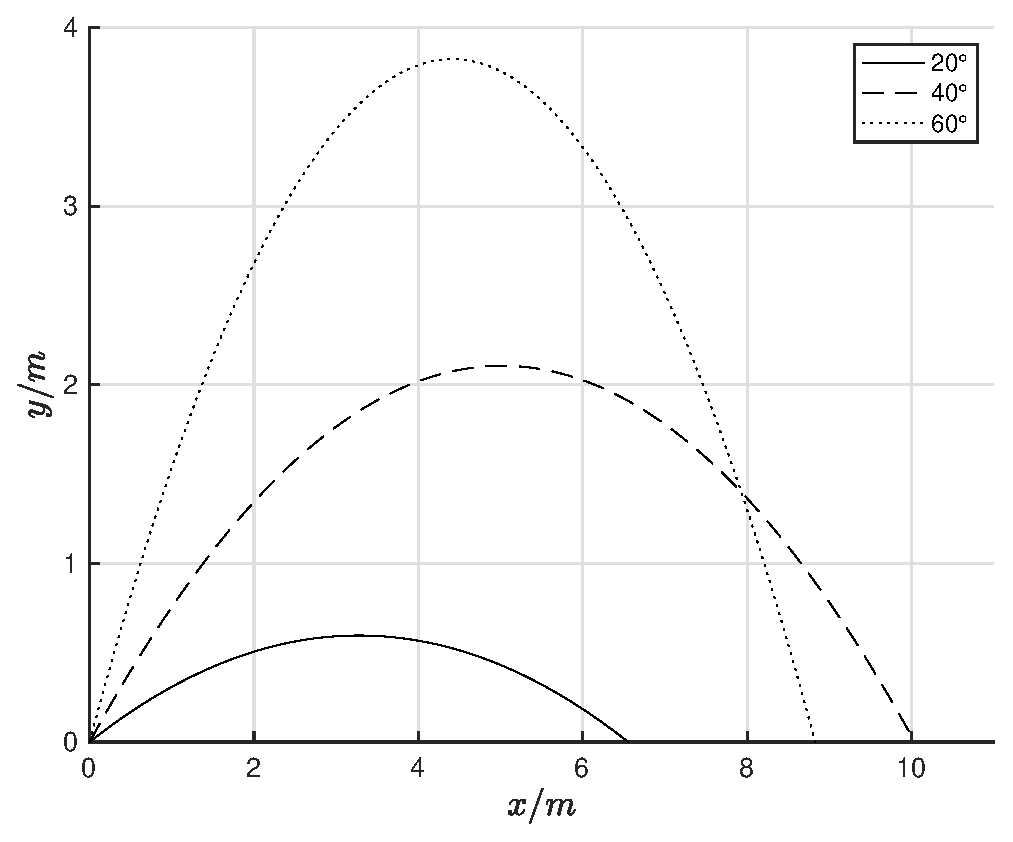
\includegraphics[scale=0.5]{Resources/Graphics/fig2_1.eps}
    \caption{BESKRIVNING}
    \label{fig:2_1}
\end{figure}

\np
\subsection*{MatLab kod}
\lstinputlisting[caption={\quad}] {Resources/Code/2.m}
\np

% Problem 3
\stepcounter{ProblemCounter}

\pagenumbering{arabic} % Start numbering
\setcounter{figure}{0} % Reset figure numbering
\setcounter{equation}{0} % Reset equation numbering
\setcounter{lstlisting}{0} % Reset code numbering

\begin{center}
    \vspace*{1cm}
    \LARGE
    \textbf{Inlämningsuppgift \arabic{ProblemCounter}}
    
    \Large
    \vspace{0.5cm}
        Fysik - Mekanik och vågor (FAFA01)
    \vspace{0.7cm}
    
    \normalsize
    \textbf{Alexandra Annedotter}
    \\
    \textbf{Georgij Michaliutin}
    
    \vspace{0.5cm}
    Utskriftsdatum: \today
 
    \vspace{1cm}
\end{center}
\section*{\centering Elliptisk satellitbana}


... Keplers andra lag... (p.371)

\begin{equation}
    v_a r_a = v_p r_p
\end{equation}

\begin{equation} \label{eq:v_min}
    v_a = \dfrac{r_p}{r_a}v_{p}
\end{equation}

...=2800 m/s 

\begin{figure}[H]
    \centering
    \captionsetup{justification=centering,margin=2cm}
    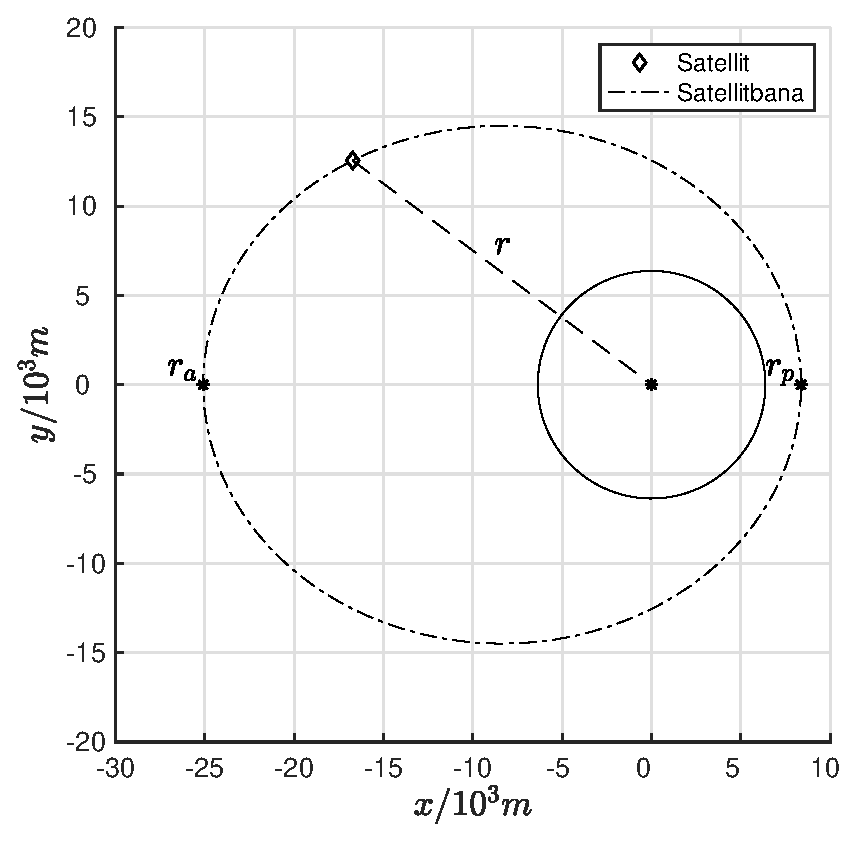
\includegraphics[scale=0.5]{Resources/Graphics/fig3_1.eps}
    \caption{BESKRIVNING}
    \label{fig:3_1}
\end{figure}

\np
\subsection*{MatLab kod}
\lstinputlisting[caption={\quad}] {Resources/Code/3.m}
\np

% Problem 4
\stepcounter{ProblemCounter}

\pagenumbering{arabic} % Start numbering
\setcounter{figure}{0} % Reset figure numbering
\setcounter{equation}{0} % Reset equation numbering
\setcounter{lstlisting}{0} % Reset code numbering

\begin{center}
    \vspace*{1cm}
    \LARGE
    \textbf{Inlämningsuppgift \arabic{ProblemCounter}}
    
    \Large
    \vspace{0.5cm}
        Fysik - Mekanik och vågor (FAFA01)
    \vspace{0.7cm}
    
    \normalsize
    \textbf{Alexandra Annedotter}
    \\
    \textbf{Georgij Michaliutin}
    
    \vspace{0.5cm}
    Utskriftsdatum: \today
 
    \vspace{1cm}
\end{center}
\section*{\centering Avbildningsfel}

\subsection*{Teori}
Detta avsnitt grundar sig på kapitel 32 i Tipler och Moscas bok \textit{Physics for Scientists and Engineers} (2008).
\vspace{5mm}

I verkligheten fokuserar inte konvexa linser ljus i exakt samma punkt. Skärningspunkten för strålar från olika vinklar och av olika våglängder varierar på grund av linsens form och material. Varierande skärningspunkt på grund av våglängd kallas \emph{kromatisk aberration}, medan varierande skärningspunkt på grund av avstånd mellan linsens centrumlinje och punkt där ljusstrålen träffar linsen kallas \emph{sfärisk aberration}. 

Ljusets brytning i en sfärisk yta beskrivs av ekvation 1.
\begin{equation}
    \dfrac{n_{luft}}{s}+\dfrac{n_{glas}}{s'} =
    \dfrac{n_{glas} - n_{luft}}{R}
\end{equation}
$n$ är brytningsindex för medium, $R$ är krökningsradien, $s$ är avstånd från ljuskälla till optisk axel, och $s'$ är avståndet från glasytans centrum till ljusets skärningspunkt ($f_b$) med den optiska axeln.

Eftersom ljusstrålar infaller parallellt med varandra (då avståndet från ljuskälla till lins antas vara stort i förhållande till våglängd) så går $s \rightarrow \infty$ vilket innebär att $\dfrac{n_{luft}}{s} \rightarrow 0$. Detta ger

\begin{equation}
    \dfrac{n_{glas}}{s'} =
    \dfrac{n_{glas} - n_{luft}}{R}.
\end{equation}
$s'$ kan ersättas med $f_b$ och ekvation 2 kan skrivas om till en formel för skärningspunkten;

\begin{equation} \label{eq:f_b}
    f_b =
    \dfrac{Rn_{glas}}{n_{glas} - n_{luft}}.
\end{equation}

Problemet kan ställas upp geometrisk som i Figur~\ref{fig:4_2}.
%för att hitta skärningspunkt inne i en sfärisk lins beroende på avståndet från linsens centrumlinje till punkten där ljusstråle träffar linsen ($h$). 

\begin{figure}[H]
    \centering
    \captionsetup{justification=centering,margin=2cm}
    \includegraphics[scale=0.7]{Resources/Graphics/fig4_2.eps}
    \caption{Geometrisk representation av sfärisk lins: $R$ = krökningsradie med centrum i $C$. Den tjocka linjen representerar en ljusstråle som träffar linsen med infallsvinkeln $\theta_1$ på avstånd $h$ från centrallinjen och har refraktionsvinkel $\theta_2$ inne i linsen. Ljusstrålen har skärningspunkt i $f$. $L$ = avståndet i x-led mellan den punkt på glasytan där ljusstrålen träffar och $f$}.
    \label{fig:4_2}
\end{figure}

Formel för brytning i plan yta:
%%där $\theta_1$, brytningsvinkel $\theta_2$:
\begin{equation} \label{eq:n_luft}
    n_{luft}\text{sin}\theta_1 = n_{glas} \text{sin}\theta_2
\end{equation}

Enligt Figur~\ref{fig:4_2} gäller
\begin{equation} \label{eq:tan_alpha}
    \text{tan}\alpha = \dfrac{h}{2L},
\end{equation}
där 
\begin{equation} \label{eq:alpha}
    \alpha = |\theta_1 - \theta_2|,
\end{equation}
där

\begin{center}
    $-\dfrac{\pi}{2}<\theta_1 <\dfrac{\pi}{2}$
    \quad och \quad
    $\dfrac{n_{luft}}{n_{glas}} < 1$
    \quad leder till \quad $|\theta_1| > |\theta_2|$.
\end{center}
Ekvation~\ref{eq:tan_alpha} och \ref{eq:alpha} ger

\begin{equation} \label{eq:L}
    L = \dfrac{h}{2\text{tan}(\theta_1-\theta_2)}.
\end{equation}

Om $\theta_2$ löses ut i ekvation 4 och detta uttryck sedan sätts in i ekvation 7 så blir
\begin{equation} \label{eq:L_2}
    L = \dfrac{h}{2\text{tan}\left(\theta_1-
    \text{arcsin}\left(\dfrac{n_{luft}}{n_{glas}}
    \text{sin}\theta_1\right)\right)}
\end{equation}


Position för skärningspunkt $f$ erhålls genom att addera $L$ ($L$ visas i Figur 1) med $R-a$ ($a$ visas i Figur 2).
\begin{equation} \label{eq:focal}
    f = L + (R-a)
\end{equation}
\begin{figure}[H]
    \centering
    \captionsetup{justification=centering,margin=2cm}
    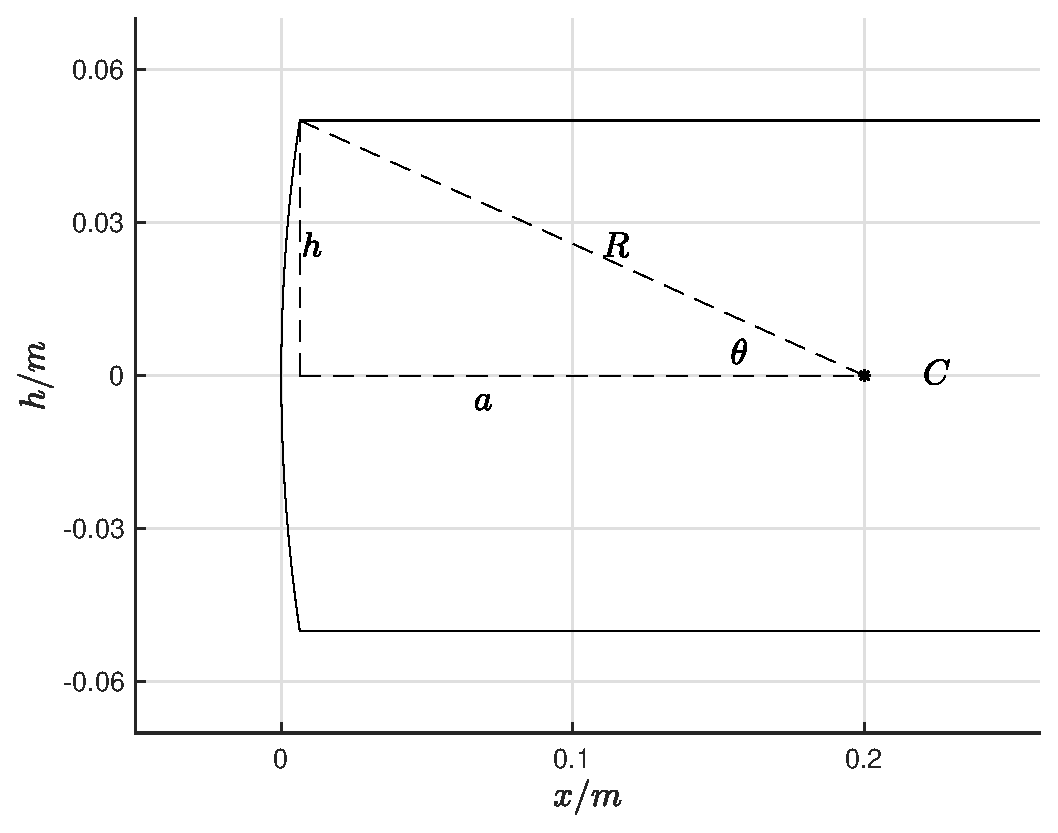
\includegraphics[scale=0.7]{Resources/Graphics/fig4_1.eps}
    \caption{Geometrisk representation av sfärisk lins: $R$ = krökningsradie med centrum i $C$, $a$ = avstånd i x-led mellan $C$ och punkten (som i y-led är $h$ m från centrallinjen) där ljusstrålen träffar linsen.}
    \label{fig:4_1}
\end{figure}


$R-a$ är det ''lilla avståndet'' i Figur 2 mellan glasytans centrum och den punkt som ligger längst till vänster på sträckan $a$. $a$ beräknas enligt
\begin{equation} \label{eq:a} 
    a = \sqrt{R^2-\dfrac{h^2}{4}}
\end{equation}

\subsection*{Resultat}
Sfärisk aberration presenteras i Figur~\ref{fig:4_3}. Kromatisk aberration i BK7-glas presenteras i Figur~\ref{fig:4_4}~och~\ref{fig:4_5}.
%%% Fig x2
\begin{figure}[H]
    \minipage{0.47\textwidth}
        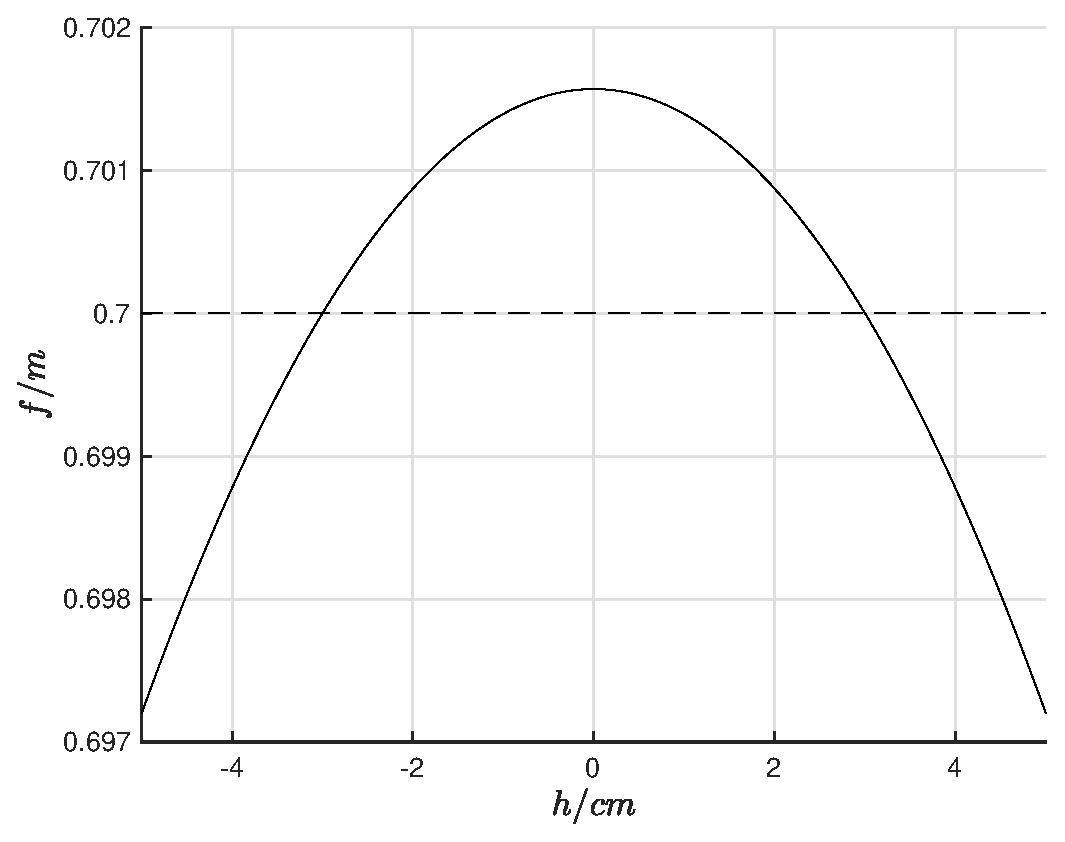
\includegraphics[width=\linewidth]{Resources/Graphics/fig4_3.eps}
        \caption{Hel linje: Skärningspunkt $f$ i meter som funktion av avståndet $h$ i cm mellan linsens centrumlinje och punkten där ljusstrålen träffar glasytan. Streckad linje: Approximation av $f$ (ekvation~\ref{eq:f_b}).}\label{fig:4_3}
    \endminipage\hfill
    \minipage{0.47\textwidth}
        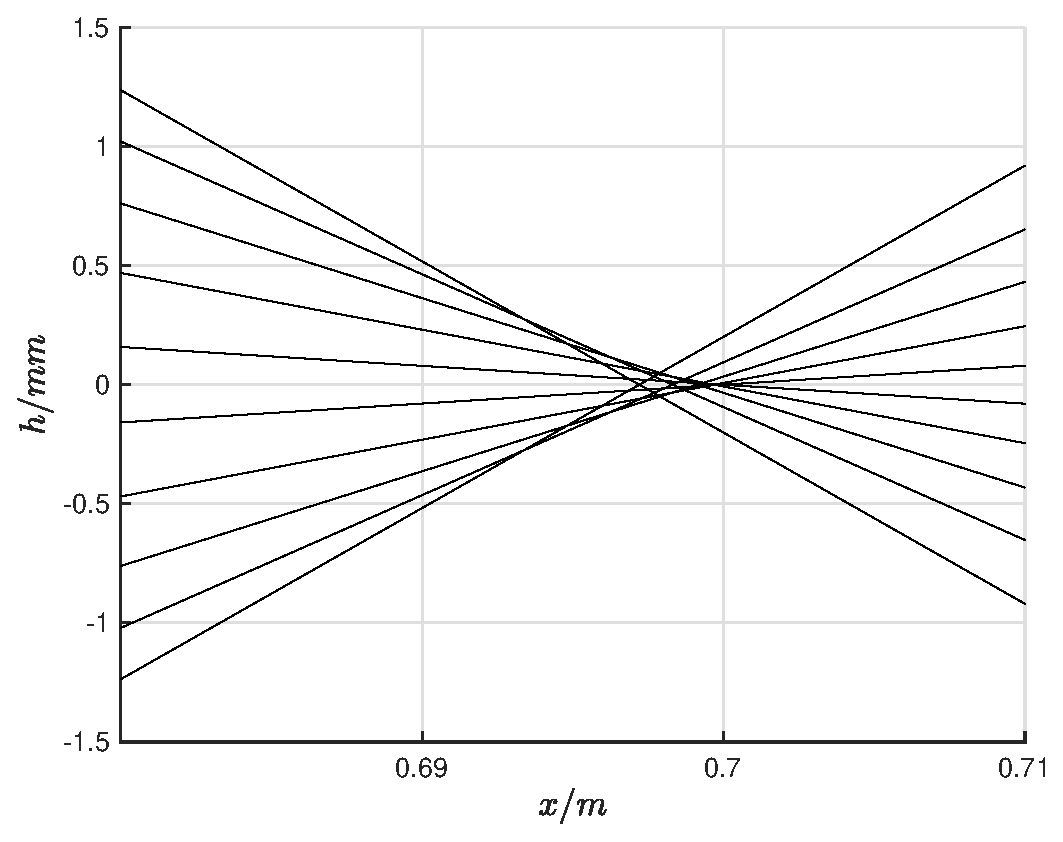
\includegraphics[width=\linewidth]{Resources/Graphics/fig4_3_2.eps}
        \caption{Visualisering av sfärisk aberration. 10 strålar som träffar linsen olika avstånd $h$ från centrumlinjen och möts inne i sfärisk lins på olika avstånd.}\label{fig:4_3_2}
    \endminipage
\end{figure}
%%% Fig x2
\begin{figure}[H]
    \minipage{0.47\textwidth}
        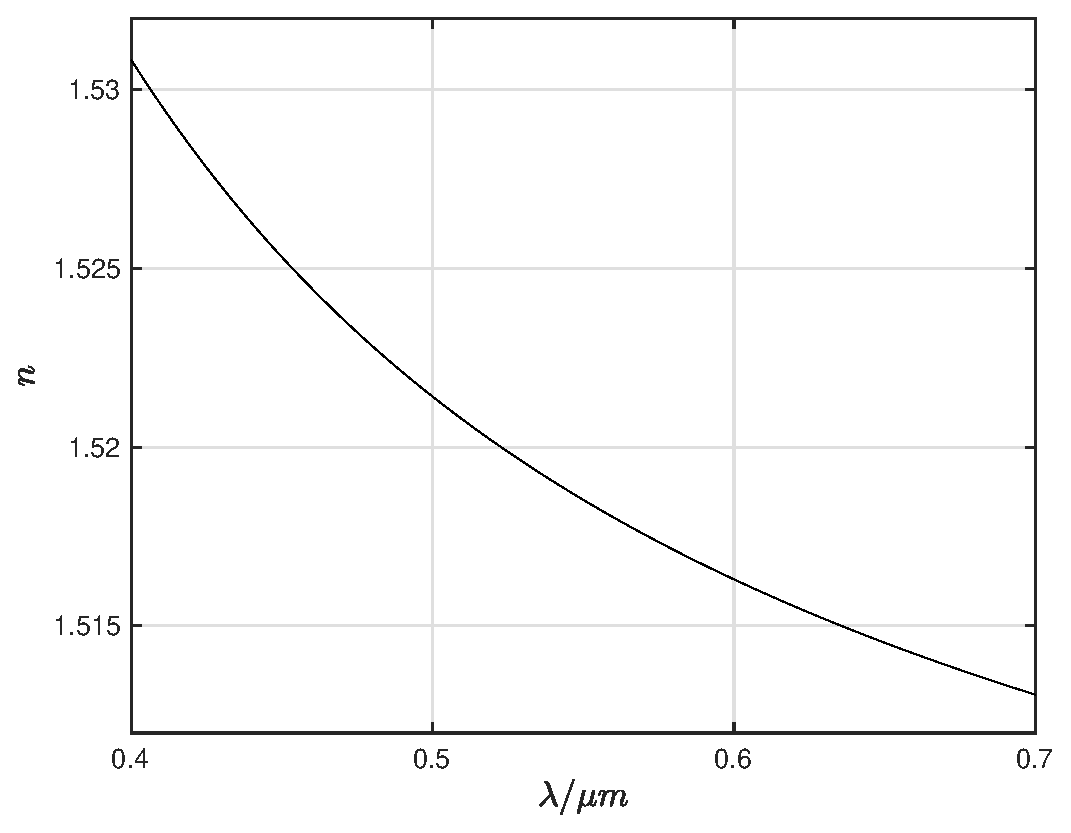
\includegraphics[width=\linewidth]{Resources/Graphics/fig4_4.eps}
        \caption{Brytningsindex $n$ som funktion av våglängd $\lambda$ för glassorten BK7.}\label{fig:4_4}
    \endminipage\hfill
    \minipage{0.47\textwidth}
        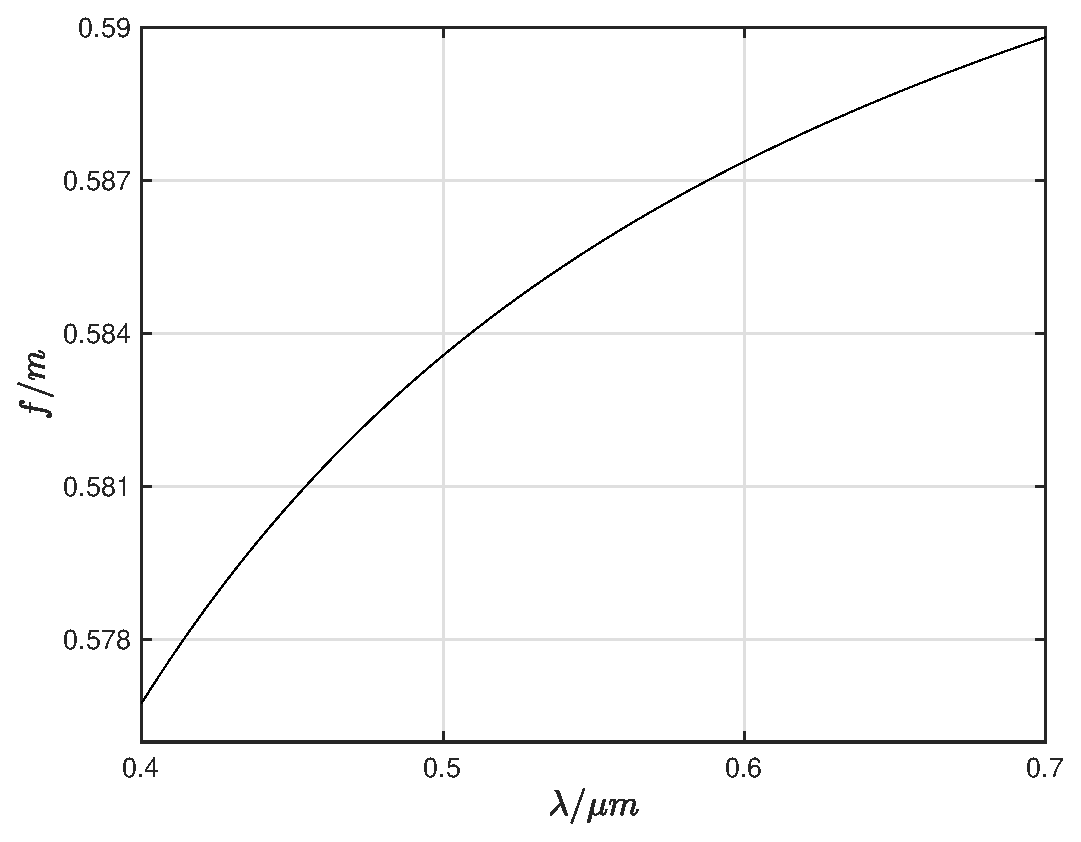
\includegraphics[width=\linewidth]{Resources/Graphics/fig4_5.eps}
        \caption{Skärningspunkt $f$ som funktion av våglängd $\lambda$ för ljusstråle med krökningsradie 0,2 m i BK7-glas.}\label{fig:4_5}
    \endminipage
\end{figure}

\subsection*{Kommentarer}
I Figur~\ref{fig:4_3} syns det tydligt att det uppstår sfärisk aberration. Ekvation~\ref{eq:f_b} ger en ganska duglig approximation av skärningspunkten $f$ då den största avvikelse (sker då $h = d/2$) ligger under 0,5\%.
\vspace{3mm}

I Figur~\ref{fig:4_4} syns det inte så stor skillnad i brytningsindex mellan synliga våglängder, detta kan förklaras med att BK7-glas har högt \emph{Abbetal} i jämförelse med andra glassorter. Desto högre Abbetal desto mindre kromatisk aberration. $[2]$ % Its a hack!

\subsection*{Referenser}
$[1]$ Mosca, Gene; Tipler, A., Paul. 2008. \textit{Physics for Scientists and Engineers}. 6:e upplagan. W.H. Freeman and Company, New York.
\vspace{2mm}

$[2]$ \textit{Optical constants of BK7},   \url{https://refractiveindex.info/?shelf=glass&book=BK7&page=SCHOTT}

\np
\subsection*{MatLab-kod}

\lstinputlisting[caption={\quad Funktion som plottar linsen}] {Resources/Code/lens_plot.m}
\lstinputlisting[caption={\quad},firstline=2] {Resources/Code/4.m}
\np

% Problem 5
\stepcounter{ProblemCounter}

\pagenumbering{arabic} % Start numbering
\setcounter{figure}{0} % Reset figure numbering
\setcounter{equation}{0} % Reset equation numbering
\setcounter{lstlisting}{0} % Reset code numbering

\begin{center}
    \vspace*{1cm}
    \LARGE
    \textbf{Inlämningsuppgift \arabic{ProblemCounter}}
    
    \Large
    \vspace{0.5cm}
        Fysik - Mekanik och vågor (FAFA01)
    \vspace{0.7cm}
    
    \normalsize
    \textbf{Alexandra Annedotter}
    \\
    \textbf{Georgij Michaliutin}
    
    \vspace{0.5cm}
    Utskriftsdatum: \today
 
    \vspace{1cm}
\end{center}
\section*{\centering Diffraktion i en spalt respektive en cirkulär apertur}
\end{document}